\begin{marginfigure}[6cm]
\margingraphics{figures/7_2_Act2_1.eps}
\end{marginfigure}

\begin{marginfigure}[1cm]
\margingraphics{figures/7_2_Act2_2.eps}
\end{marginfigure}

\begin{activity} \label{A:7.2.1}  
Consider the autonomous differential equation 
$$ \frac{dy}{dt} = -\frac 12 y(y-4). $$

\ba
\item Make a plot of $\frac{dy}{dt}$ versus $y$.  Looking at the
  graph, for what values of $y$ does $y$ increase and for what values of $y$
  does $y$ decrease?

\item Identify any equilibrium solutions of the given differential equation.

\item Now sketch the slope field for the given differential equation.

\item  Sketch the solutions to the given differential equation that correspond to initial values $y(0)=-1, 0, 1, \ldots, 5$.

\item  An equilibrium solution $\overline{y}$ is called {\em stable} \index{stable} \index{equilibrium solution!stable}
  if nearby 
  solutions converge to $\overline{y}$.  This means that if the inital
  condition varies slightly from $\overline{y}$, then
  $\lim_{t\to\infty}y(t) = \overline{y}$.  

  Conversely, an equilibrium solution $\overline{y}$ 
  is called {\em unstable} \index{unstable} \index{equilibrium solution!unstable} if nearby solutions are pushed away from
  $\overline{y}$.

  Using your work above, classify the equilibrium solutions you found in (b)
  as either stable or unstable.

\item Suppose that $y(t)$ describes the population of a species of
  living organisms and that the initial value $y(0)$ is positive.  What can you
  say about the eventual fate of this population?  

\item  Remember that an equilibrium solution $\overline{y}$ satisfies
  $f(\overline{y}) = 0$.  If we graph $dy/dt = f(y)$ as a function of
  $y$, for which of the following differential equations is
  $\overline{y}$ a stable equilibrium and for which is $\overline{y}$ unstable?  Why?

  \begin{center}
    \includegraphics{figures/7_2_Act2_3.eps} \qquad
    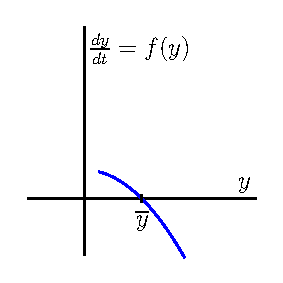
\includegraphics{figures/7_2_Act2_4.eps} 
  \end{center}

\ea
\end{activity}
\begin{smallhint}
\ba
	\item Small hints for each of the prompts above.
\ea
\end{smallhint}
\begin{bighint}
\ba
	\item Big hints for each of the prompts above.
\ea
\end{bighint}
\begin{activitySolution}
\ba
	\item Solutions for each of the prompts above.
\ea
\end{activitySolution}
\aftera